\documentclass[a4paper,12pt]{report}
\usepackage[utf8]{inputenc}
\usepackage{graphicx}
\usepackage{amsmath}
\usepackage{amsfonts}
% \usepackage[bitstream-charter]{mathdesign}
% \usepackage[T1]{fontenc}

\usepackage{hyperref}
\usepackage{cite}
\usepackage{lipsum}
\usepackage[margin=2.5cm]{geometry}
\usepackage{setspace}
\usepackage{float}
\graphicspath{ {./figures/} }

\onehalfspacing

\newtheorem{definition}{Definition}
\newtheorem{remark}{Remark}

\title{BSc Thesis}
\author{Edoardo Ghirardo}
\date{\today}

\hypersetup{
    colorlinks=true,
    linkcolor=black,
    citecolor=black,
    filecolor=black,
    urlcolor=black
}

\begin{document}

\pagenumbering{gobble} % Suppress page numbers initially

\cleardoublepage % Add blank page after title
\null\thispagestyle{empty}
\cleardoublepage % Add second blank page
\null\thispagestyle{empty}

\chapter*{Acknowledgements}



\cleardoublepage % Add second blank page
\null\thispagestyle{empty}

\pagenumbering{arabic} % Start page numbering in arabic numerals

\tableofcontents

\chapter{Introduction}\label{ch:introduction}
The relationship between physics and finance is a long-standing one. \cite{bachelier} is perhaps the first example of a model developed by physicists, in this case Brownian motion, being applied to financial markets, specifically to the pricing of derivative products. This work would remain largely unnoticed until \cite{black_scholes} was published, which is now considered the foundation of modern quantitative finance.

Beyond derivative pricing, econophysics as a field has been active since the 1990s, with the aim of applying methods from statistical physics to a wide range of problems in economics and finance. \cite{bouchaud_mezard_2000}, for instance, examines the distribution of wealth in a simplified model of an economy, mapping this problem to the random `directed polymer' problem.

For an introduction to the field of econophysics, refer to  \cite{Mantegna_Stanley_1999} and \cite{econophysics_2011_review}.

\section{Motivation}
The scope of this work is to review the spin model of financial price introduced in \cite{bornholdt}, after going through the relevant core background in statistical physics. From simulations (\textcolor{red}{and analytical results?}), we will see that the price time-series generated by this model exhibits properties similar to those observed in real financial data, challenging the assumptions of commonly used financial models. 


\chapter{Background and theoretical framework}
\label{ch:background}

\section{Financial mathematics: option pricing}
\label{sec:financial_background}
\textcolor{red}{to be expanded: introduction}\\
In this section, we will first provide a brief introduction to the language of financial mathematics in continuous time, and then introduce the Black-Scholes model for option pricing.

\subsection{Setting and no-arbitrage theory}
Let us assume we have a financial market on which a bond $B$ and a stock $S$ are traded. We will describe the dynamics of the price of each asset in a continuous time setting. We will assume that the bond $B$ has a deterministic return $r$:
\begin{equation}
    \label{eq:bond}
    dB(t) = r B(t) dt
\end{equation}
On the other hand, we will assume that the stock $S$ follows a geometric Brownian motion:
\begin{equation}
    \label{eq:stock}
    dS(t) = \mu S(t) dt + \sigma S(t) dW(t)
\end{equation}
Where $W(t)$ is a standard Brownian motion, $\mu$ is the drift, and $\sigma$ is the volatility of the stock. The drift $\mu$ is the expected return of the stock, and the volatility $\sigma$ is a measure of the uncertainty of the stock price.

We can now go ahead and define what a european call option is.
\begin{definition}
    A european call option is a contract that gives the holder the right, but not the obligation, to buy an asset at a specified price (the strike price) at a specified time (the expiration date). The payoff of a european call option at time $t$ is given by:
    \begin{equation}
        X(t) = \begin{cases}
            max(S(t)-K,0) & \text{if } t = T\\
            0 & \text{if } t < T
        \end{cases}
    \end{equation}
    Where $S(t)$ is the price of the underlying asset at time $t$, $K$ is the strike price, and $T$ is the expiration date. The payoff is zero if the option is not exercised, and it is equal to the difference between the price of the underlying asset and the strike price if the option is exercised.
\end{definition}

The question we want to answer is: what is the fair price of a european call option? In order to answer this question, we will need to introduce the concept of no-arbitrage. The idea is that if we can find a way to make a profit without any risk, then we can use this strategy to make money. This is not possible in a well-functioning market, so we will assume that there are no arbitrage opportunities.

Let us define $C(t)$ as the price of a european call option with expiration $T$ and strike price $K$. We will then work on the market $\mathcal{M} = \{B(t),S(t),C(t)\}_{t\in\mathcal{T}}$, where $\mathcal{T}$ is the set of trading times. On this market, a portfolio $h(t) = \{h_B(t),h_S(t),h_C(t)\}$ is defined as the number of units of each asset held at time $t$. The value of the portfolio at time $t$ is given by:
\begin{equation}
    V^h(t) = h_B(t)B(t) + h_S(t)S(t) + h_C(t)C(t)
\end{equation}
Now, we can define the concepts of self-financing portfolio and arbitrage opportunity.
\begin{definition}
    A portfolio is said to be self-financing if the value process of the portfolio satisfies the following equation:
    \begin{equation}
        dV^h(t) = h_B(t)dB(t) + h_S(t)dS(t) + h_C(t)dC(t)
    \end{equation}
    This means that the change in the value of the portfolio is equal to the sum of the changes in the value of each asset, weighted by the number of units held in each asset. Intuitively, a self-financing portfolio is one in which the changes in the value of the portfolio are due to the changes in the value of the assets, and not due to any additional investments or withdrawals.
\end{definition}
\begin{definition}
    An arbitrage opportunity is a self-financing portfolio $h(t)$ such that the following conditions hold:
    \begin{enumerate}
        \item $V^h(0) = 0$.
        \item $P(V^h(T) \geq 0) = 1$.
        \item $P(V^h(T) > 0) > 0$.
    \end{enumerate}
    Meaning that the portfolio has zero initial value, it is non-negative at time $T$, and it has a positive probability of being strictly positive at time $T$. Intuitively, an arbitrage opportunity is a way to make a sure profit without any initial investment.
\end{definition}

\begin{lemma}
    \label{lem:risk_free}
    Suppose that in an arbitrage-free market there exists a self-financing portfolio $h(t)$ such that $dV^h(t) = k V^h(t) dt$, where $k$ is a constant. Then, the return $k$ is equal to the risk-free rate $r$.
\end{lemma}
\begin{proof}
    Assume WLOG $B(0) = 1$. Assume $V^h(0) > 0$ and $k>r$. Other cases are either equivalent or equivalent by reversing the position.
    Let us construct a portfolio $h'(t)$ consisting of one unit of the self-financing portfolio $h(t)$ and $-V^h(0)$ units of the risk-free asset $B(t)$, such that:
    \begin{equation}
        V^{h'}(0) = V^h(0)-V^h(0) = 0
    \end{equation}
    And for $t>0$:
    \begin{equation}
        \begin{aligned}
            V^{h'}(t) &= V^h(t) - V^h(0)B(t)\\
            &= V^h(0)e^{kt} - V^h(0)e^{rt}\\
            &= V^h(0)(e^{kt} - e^{rt}) > 0
        \end{aligned}
    \end{equation}
    Which makes $h'(t)$ an arbitrage opportunity, which is a contradiction. Therefore, we must have $k = r$.
\end{proof}
% \textcolor{red}{change to continuous time}\\s
% Let $\mathcal{T}$ be the set of trading times, and let $\Omega$ be the state space of the price of a stock. Let $\mathcal{P} = \{\mathcal{P}_t\}_{t\in\mathcal{T}}$ be a filtration on $\Omega$. On this setting, we can define a locally riskless asset $\{B(t)\}_{t\in\mathcal{T}}$, described by a $\mathcal{P}_t$-measurable stochastic process $\{r(t)\}_{t\in\mathcal{T}}$, which is the return of $B(t)$ at time $t$. The return is defined as:
% \begin{equation}
%     r(t) = \frac{B(t+1)-B(t)}{B(t)} \quad \forall t\in\mathcal{T}
% \end{equation}
% We can also define N risky assets as $\mathcal{P}_{t+1}$-measurable stochastic processes $\{S_i(t)\}_{t\in\mathcal{T}} \; i\in \{1,\dots,N\}$, which is the price of each asset at time $t$. Intuitively, the locally riskless asset is a bond, for which we know the return at time $t+1$ given the return at time $t$. The risky assets are stocks, for which we do not know the return at time $t+1$ given the return at time $t$.

% % fix to make it continous time!!

% % Let $\theta_j = \{\theta_j(t)\}_{t\in\mathcal{T}}$ be stochastic process representing the value of the position held in the j-th asset, which might be positive or negative (in the case of short selling).

% \textcolor{red}{TBA: definition of no arbitrage}



% A european put option is defined similarly, as the right to sell an asset at a specified price at a specified time.

\subsection{The Black-Scholes model}
\subsubsection{Assumptions}
The Black-Scholes model is a mathematical model for the pricing of european options, introduced in \cite{black_scholes}. The assumptions for deriving the price of the option are:
\begin{enumerate}
    \item There exists a locally riskless asset with known and constant return, as we introduced it in Equation~\ref{eq:bond}: 
    $$
        dB(t) = r B(t) dt
    $$
    Where $r$ is the risk-free return.
    \item  \label{it:gbm}The risky asset follows a geometric Brownian motion, as we untroduced it in Equation~\ref{eq:stock}:
    $$
        dS(t) = \mu S(t) dt + \sigma S(t) dW(t)
    $$
    Where $W(t)$ is a standard Brownian motion, $\mu$ is the constant drift, and $\sigma$ is the volatility of the asset.
    \item The market is frictionless, meaning that there are no transaction costs, and the assets can be traded continuously.
    \item The asset pays no dividends.
    \item It is possible to short-sell the asset without any restrictions or penalties.
    \item It is possible to borrow a fraction of the security at the risk-free rate.
\end{enumerate}

\subsubsection{Derivation}
Let \( C(S,t) \) be the price of a European call option written on the underlying asset \( S(t) \).

Applying Itô's Lemma to \( C(S,t) \), we have:
\[
dC = \frac{\partial C}{\partial t} dt + \frac{\partial C}{\partial S} dS + \frac{1}{2} \frac{\partial^2 C}{\partial S^2} dS^2
\]

Substitute the dynamics of \( S(t) \):
\[
dS = \mu S dt + \sigma S dW
\]
\[
dS^2 = (\sigma S)^2 dt = \sigma^2 S^2 dt
\]

Thus:
\[
dC = \frac{\partial C}{\partial t} dt + \frac{\partial C}{\partial S} (\mu S dt + \sigma S dW) + \frac{1}{2} \frac{\partial^2 C}{\partial S^2} \sigma^2 S^2 dt
\]

Simplify:
\[
dC = \left( \frac{\partial C}{\partial t} + \mu S \frac{\partial C}{\partial S} + \frac{1}{2} \sigma^2 S^2 \frac{\partial^2 C}{\partial S^2} \right) dt + \sigma S \frac{\partial C}{\partial S} dW
\]

Now, construct a hedged portfolio \( \Pi = C - \Delta S \), where \( \Delta = \frac{\partial C}{\partial S} \). The change in the portfolio is:
\[
d\Pi = dC - \Delta dS
\]

Substituting:
\[
d\Pi = \left( \frac{\partial C}{\partial t} + \frac{1}{2} \sigma^2 S^2 \frac{\partial^2 C}{\partial S^2} \right) dt
\]

Note that the \( dW \) terms cancel because:
\[
\sigma S \frac{\partial C}{\partial S} dW - \frac{\partial C}{\partial S} \sigma S dW = 0
\]

This portfolio is riskless, and by Lemma~\ref{lem:risk_free}, it must grow at the risk-free rate:
\[
d\Pi = r \Pi dt = r(C - \Delta S) dt
\]

Equating both expressions for \( d\Pi \):
\[
\left( \frac{\partial C}{\partial t} + \frac{1}{2} \sigma^2 S^2 \frac{\partial^2 C}{\partial S^2} \right) dt = r \left( C - S \frac{\partial C}{\partial S} \right) dt
\]

Cancelling \( dt \) and rearranging terms:
\[
\frac{\partial C}{\partial t} + \frac{1}{2} \sigma^2 S^2 \frac{\partial^2 C}{\partial S^2} + r S \frac{\partial C}{\partial S} - rC = 0
\]

This is the Black-Scholes partial differential equation (PDE).

\subsubsection{Formula}

The Black-Scholes formula for a European call option with strike price \( K \), time to maturity \( T - t \), and current underlying price \( S \) is:

\[
C(S,t) = S \Phi(d_1) - K e^{-r(T - t)} \Phi(d_2)
\]

where:
\[
d_1 = \frac{\ln(S/K) + (r + \frac{1}{2} \sigma^2)(T - t)}{\sigma \sqrt{T - t}}, \quad
d_2 = d_1 - \sigma \sqrt{T - t}
\]

and \( \Phi(\cdot) \) is the cumulative distribution function of the standard normal distribution.

\subsection{Discussion}
The Black-Scholes model relies on several key assumptions, one of which is that the price of the underlying asset follows a geometric Brownian motion with constant volatility. While this assumption is mathematically convenient and allows for an analytical solution to the pricing problem, it does not always align with empirical observations of financial markets.

In practice, the distribution of asset returns often exhibits fat tails, meaning that extreme events (large positive or negative returns) occur more frequently than predicted by a normal distribution. Furthermore, returns are not always independent over time; they often exhibit autocorrelation, which violates the assumption of independent increments in the geometric Brownian motion.

These discrepancies have significant implications. For instance, the assumption of normally distributed returns can lead to an underestimation of the probability and impact of extreme market events, such as the 1987 stock market crash, the 2008 financial crisis, or the COVID-19 pandemic-induced market turmoil. Such underestimations can result in inadequate risk management strategies.

Given the widespread use of the Black-Scholes model and its extensions in the financial industry, particularly in the pricing of derivatives, understanding the limitations of its assumptions is crucial. According to \cite{bis}, the notional value of the over-the-counter derivatives market has reached approximately \$730 trillion. This highlights the potential global impact of mispricing and underestimating risks due to unrealistic assumptions.

To address these limitations, alternative models have been proposed that aim to capture more realistic dynamics of asset prices. One promising approach is to model price movements based on the interplay of supply and demand, which is driven by the collective behavior of market participants. This perspective naturally leads to the study of models inspired by statistical physics, where the interactions of many agents are explicitly considered. In the next section, we will introduce key concepts from statistical physics to formalize this approach.


\section{Statistical physics: the Ising model}
In this section, we introduce the Ising model as an example of model driven by the interaction of many agents (spins). The Ising model is a simple mathematical model of ferromagnetic materials. In its description, we will mostly follow the notation and tools presented in \cite{mezard_book} and from professor Mézard's lecture notes. The model consists of Ising spins (that is, spins which can take binary values) on a d-dimensional cubic lattice (see figure \ref{fig:ising_model}). Mathematically, given a cubic lattice $\mathbb{L}=\{1,\dots,L\}^n$, we define an an Ising spin $\sigma_i\in\{-1,1\}$ for each site $i\in\mathbb{L}$. Then, we can have any configuration $\underline{\sigma} = (\sigma_1,\dots,\sigma_n) \in \mathcal{X}_N=\{+1,-1\}^{\mathbb{L}}$.

\begin{figure}[h]
    \centering
    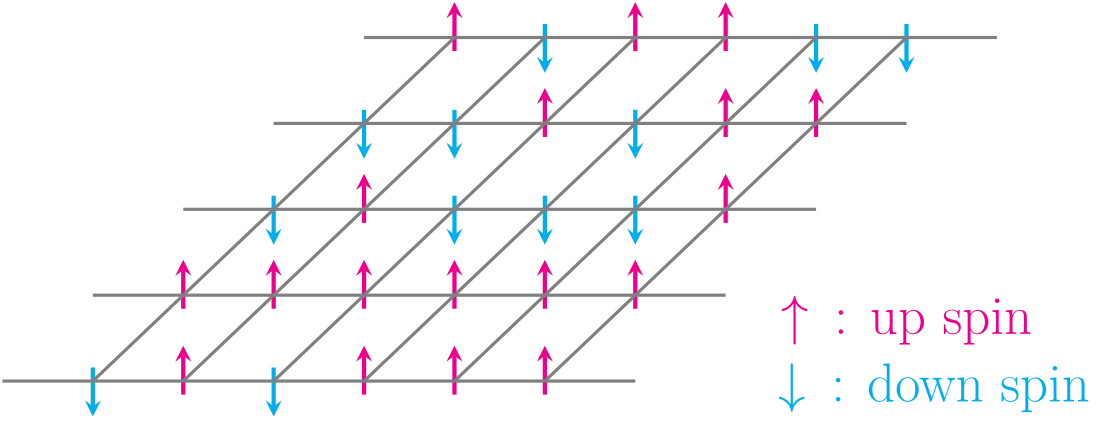
\includegraphics[width=0.5\textwidth]{2D_ising_model_on_lattice.svg.png}
    \caption{The Ising model on a 2D lattice.}
    \label{fig:ising_model}
\end{figure}


The energy of a configuration $\underline{\sigma}$ is given by:
\begin{equation}
    H(\underline{\sigma}) = -\sum_{\langle i,j\rangle}\sigma_i\sigma_j - B\sum_i \sigma_i
\end{equation}
Where the sum over $\langle i,j\rangle$ is a sum over all nearest neighbors, and $B$ is an external magnetic field. At equilibrium, the probability of a configuration $\underline{\sigma}$ is given by the Boltzmann distribution:
\begin{equation}
    P(\underline{\sigma}) = \frac{e^{-\beta H(\underline{\sigma})}}{Z}
\end{equation}
Where $\beta$ is the inverse temperature, and $Z$ is the partition function:
\begin{equation}
    Z = \sum_{\underline{\sigma}\in\mathcal{X}_N}e^{-\beta H(\underline{\sigma})}
\end{equation}
Interestingly, despite its simplicity, an analytical, closed-form solution for \(Z\) has been found only in the $d=1$ and $d=2$ cases. Higher dimensions remain unsolved, but numerical methods and mean-field approximations can be used to study the model in these cases.

One important quantity in the Ising model is the magnetization, which is defined as:
\begin{equation}
    m = \frac{1}{N}\sum_i \langle \sigma_i \rangle
\end{equation}
where $\langle \cdot \rangle$ denotes the average.

\subsection{Solution of the Ising model in the one-dimensional case}
For simplicity, assume $B=0$. In the one-dimensional case, the Ising model can be solved exactly. Recall that:
\begin{equation}
    H(\underline{\sigma}) = -\sum_{\langle i,j\rangle}\sigma_i\sigma_j
\end{equation}
Then, the partition function is given by:
\begin{equation}
    Z = \sum_{\underline{\sigma}\in\mathcal{X}_N}e^{-\beta H(\underline{\sigma})} =
    \sum_{\underline{\sigma}\in\mathcal{X}_N}e^{\beta\sum_{\langle i,j\rangle}\sigma_i\sigma_j}
\end{equation}
Since each spin is connected to its nearest neighbors, we can write:
\begin{equation}
    Z =  \sum_{\underline{\sigma}\in\mathcal{X}_N}e^{\beta\sum_n\sigma_n\sigma_{n+1}}
\end{equation}
Let us define $\tau_n = \sigma_{n-1}\sigma_{n} \implies \sigma_n = \tau_n\tau_{n-1}\dots\tau_2\sigma_1$. Then, we can write:
\begin{equation}
    \begin{gathered}
    Z =  \sum_{\sigma_1\in\{-1,1\}}\sum_{\tau_2,\dots\tau_n}e^{\beta\sum_n\tau_n}
    = 2\sum_{\tau_2,\dots,\tau_N}e^{\beta\sum_n\tau_n}\\
    = 2\sum_{\tau_2,\dots,\tau_N}\prod_n e^{\beta\tau_n}
    = 2(\sum_{\tau_2}e^{\beta\tau_2})\dots(\sum_{\tau_N}e^{\beta\tau_N})\\
    = 2(2\cosh(\beta))^{N}
    \end{gathered}
\end{equation}
Thus, we have found an analytical expression for the partition function in the one-dimensional case. The magnetization can be computed as:
\begin{equation}
    \label{eq:ising}
    m = \frac{1}{N}\sum_i \langle \sigma_i \rangle = \frac{1}{N}\frac{\partial}{\partial \beta}\log Z = \tanh(\beta)
\end{equation}
%check magnetization formula


% \subsection{Mean-field approximation of the Ising model in higher dimensions}
% While a closed-form solution for the Ising model in two dimensions exists, it does not for $d\geq 3$ so we will study its mean-field approximation. The method we will see can be applied to a more general Ising model, and then be reconduced to the original one. The hamiltonian we focus on is:
% \begin{equation}
%     H(\underline{\sigma}) = -\sum_{\langle i,j\rangle}J_{i,j}\sigma_i\sigma_j - \sum_i B_i\sigma_i
% \end{equation}
% Which differs from the standard Ising model by having arbitrary $J_{i,j}$ and $B_i$ for every $i,j$. The idea is to approzimate the Boltzmann distribution $P(\underline{\sigma}) = (1/Z)e^{-\beta H(\underline{\sigma})}$ with a probability with independent variables $Q(\underline{\sigma})= \prod_{i=1}^Nq_i(\sigma_i)$. The idea is to find the $q_i$ such that the ``distance'' between $P$ and $Q$ is minimized. We will use the Kullback-Leibler divergence as notion of distance.
% \begin{definition}
%     Given $p(x)$ and $q(x)$ probability distributions over the same finite space $\mathcal{X}$, the Kullback–Leibler (KL) divergence between them is:
%     $$D(q||p) = \sum_{x\in\mathcal{X}}q(x)\log\frac{q(x)}{p(x)}$$
% \end{definition}
% \begin{remark}
%     \hfill
%     \begin{enumerate}
%         \item $D(q||p)$ is convex in $q(x)$.
%         \item $D(q||p)\geq 0$ with equality $ \iff p(x)=q(x) \;\forall x\in\mathcal{X}$.
%         \item In general, the KL divergence is not symmetric.
%     \end{enumerate}
%     Then, the KL divergence lacks the symmetry property to be properly defined as a distance between probability distributions.
% \end{remark}
% We will define $Q$ as the most general joint binary probability distribution:
% \begin{equation}
%     Q(\underline{\sigma}) = \prod_{i=1}^{N}q_i(\sigma_i); \quad
%     q_i(\sigma_i)=\frac{1+m_i\sigma_i}{2}
% \end{equation}
% Where $m_i$ is the mean of each $q_i$, and it is the parameter which we want to find. Then,
% \begin{equation}
%     \begin{gathered}
%         D(Q||P) = \sum_{\underline{\sigma}\in\mathcal{X}}Q(\underline{\sigma})\log\frac{Q(\underline{\sigma})}{P(\underline{\sigma})}\\
%         =\sum_{\underline{\sigma}\in\mathcal{X}}Q(\underline{\sigma})\log Q(\underline{\sigma}) - \sum_{\underline{\sigma}\in\mathcal{X}}Q(\underline{\sigma})\log P(\underline{\sigma}) = (A) + (B)\\
%     \end{gathered}
% \end{equation}
% We can split this in the first term, depending only on $Q$, and the second term, depending on $P$ as well. Then:
% \begin{equation}
%     \begin{gathered}
%         (A) = \sum_{\underline{\sigma}\in\mathcal{X}}Q(\underline{\sigma})\log Q(\underline{\sigma}) = \sum_{i=1}^{N}\left(\frac{1+m_i}{2} \log \frac{1+m_i}{2}+\frac{1-m_i}{2} \log \frac{1-m_i}{2}\right)\\
%         (B) = \beta \sum_{i<j} J_{i j} m_i m_j + \beta \sum_i B_i m_i-\log Z
%     \end{gathered}
% \end{equation}
% In the second term, we see that the $\log Z$ term is independent of $m_i$, so we can ignore it. Then, we are interested in finding the values of $m_i$ that solve:
% \begin{equation}
%     \frac{\partial D(Q||P)}{\partial m_i} = 0 \iff \frac{1}{2} \log \frac{1+m_i}{1-m_i} - \beta \sum_{j\in \partial_i} J_{i j} m_j - \beta B_i = 0
% \end{equation}
% Then, we find the mean field equation:
% \begin{equation}
%     m_i = \tanh\left(\beta\sum_{j\in \partial_i} J_{i j} m_j + \beta B_i\right)
% \end{equation}
% Now, going back to the original Ising model, we can set $J_{i,j} = J$ and $B_i=B \implies m_i = m$. Then, we have the mean field equation for the Ising model in $d$ dimensions:
% \begin{equation}
%     m = \tanh(\beta (B + 2dJm))
% \end{equation}
% Let us consider the case $B=0$. Then, depending on the value of $\beta$, we can have one or three solutions to the mean-field equation, depending on the slope of the function $f(m) = \tanh(\beta 2dJm)$. The critical value of $\beta$ is then:
% \begin{equation}
%     \beta_c = \frac{1}{2dJ}
% \end{equation}

\subsection{The Curie-Weiss model}
\label{sec:curie_weiss}
The Curie-Weiss model is a generalization of the Ising model, where instead of interacting with nearest neighbors, each spin interacts with all other spins. The Hamiltonian is given by:
\begin{equation}
    H(\underline{\sigma}) = -\frac{J}{N}\sum_{i<j}\sigma_i\sigma_j - B\sum_i \sigma_i
\end{equation}
The scaling factor $\frac{1}{N}$ is introduced to have a non-trivial free energy. This model is interesting because it introduced the concept of mean-field approximations. As usual, the partition function is given by:
\begin{equation}
    \begin{aligned}
        Z &= \sum_{\underline{\sigma}\in\mathcal{X}_N}e^{-\beta H(\underline{\sigma})}\\
        &= \sum_{\underline{\sigma}\in\mathcal{X}_N}e^{\beta\frac{J}{N}\sum_{i<j}\sigma_i\sigma_j+\beta B \sum_i \sigma_i}\\
        &= \sum_{\underline{\sigma}\in\mathcal{X}_N}e^{\frac{1}{2}\beta\frac{J}{N}\sum_{i,j}\sigma_i\sigma_j+\beta B \sum_i \sigma_i-\frac{1}{2}\beta J}\\
        &= \sum_{\underline{\sigma}\in\mathcal{X}_N}e^{\frac{1}{2}\beta\frac{J}{N}\left(\sum_{i}\sigma_i\right)^2+\beta B \sum_i \sigma_i-\frac{1}{2}\beta J}\\
    \end{aligned}
\end{equation}
Now, we can introduce the notation:
\begin{equation}
m(\underline{\sigma}) = \frac{1}{N}\sum_{i}\sigma_i
\end{equation}
Then, we can rewrite the hamiltonian as:
\begin{equation}
    H(\underline{\sigma}) = \frac{1}{2} J N m^2(\underline{\sigma}) + B N m(\underline{\sigma}) - \frac{1}{2}\beta J
\end{equation}
And the partition function becomes:
\begin{equation}
    \begin{aligned}
        Z &= \sum_{\underline{\sigma}\in\mathcal{X}_N}e^{\frac{1}{2}\beta J N m^2(\underline{\sigma}) + \beta B N m(\underline{\sigma})-\frac{1}{2}\beta J}\\
        &= \sum_{m}e^{\frac{1}{2}\beta J N m^2 + \beta B N m-\frac{1}{2}\beta J}\mathcal{N}(m)\\
        &= \sum_{m}e^{N\left(\frac{1}{2}\beta J m^2 + \beta B m + \frac{1}{N}\log\mathcal{N}(m)\right)-\frac{1}{2}\beta J}
    \end{aligned}
\end{equation}
Where $\mathcal{N}(m)$ is the number of configurations with magnetization $m$. Now, we can focus on the term $\frac{1}{N} \log\mathcal{N}(m)$, which in the large $N$ limit we will call $S(m)$.
\begin{equation}
    \begin{aligned}
        S(m) &= \lim_{N \rightarrow \infty}\frac{1}{N}\log\mathcal{N}(m)\\
        &= \lim_{N \rightarrow \infty}\frac{1}{N}\log \frac{N!}{\left(\frac{1+m}{n}N\right)!\left(\frac{1-m}{n}N\right)!}\\
    \end{aligned}
\end{equation}
Since, in order to get a magnetization $m$, we need exactly $\frac{1+m}{2}N$ spins up and $\frac{1-m}{2}N$ spins down, which can happen in $\binom{N}{\frac{1+m}{2}N}$ ways. Then, since we are interested in the large $N$ limit, we can use Stirling's approximation:
\begin{equation}
    \log n! \approx n\log n - n
\end{equation}
Which allows us to rearrange and simplify the expression for $S(m)$:
\begin{equation}
    S(m) = -\frac{1+m}{2}\log\left(\frac{1+m}{2}\right) - \frac{1-m}{2}\log\left(\frac{1-m}{2}\right)
\end{equation}

Now, we recall the definition of the Shannon entropy:
\begin{definition}
    The Shannon entropy of a discrete probability distribution $p(x)$ is defined as:
    \begin{equation}
        S(p) = -\sum_x p(x)\log p(x)
    \end{equation}
    Where the sum is taken over all possible values of $x$.
    The Shannon entropy measures the amount of uncertainty or information in the distribution.
\end{definition}

And we notice that $S(m)$ is the Shannon entropy of a bernoulli distribution with probability $p = \frac{1+m}{2}$ and $q = \frac{1-m}{2}$.

Now, in the large $N$ limit, we notice the following:
\begin{itemize}
    \item The increments of $m$ become infinitesimal, allowing us to treat the sum as an integral.
    \item We can use the stirling approximation for the factorials, allowing us to subtitute $\frac{1}{N}\log\mathcal{N}(m)$ with $S(m)$.
    \item We can neglect the term $-\frac{1}{2}\beta J$ in the exponent, as it is $o(N)$.
\end{itemize}
Then, we can rewrite the partition function as:
\begin{equation}
    \label{eq:curie_weiss_phi}
    Z \approx \int_{-1}^{1} dm e^{N\phi(m)}, \quad \text{where }
    \phi(m) = \frac{1}{2}\beta J m^2 + \beta B m + S(m)
\end{equation}

\begin{figure}[h]
    \centering
    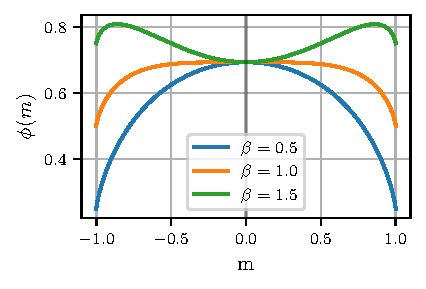
\includegraphics[width=0.49\textwidth]{curieweiss/m_phi_B0.pdf}
    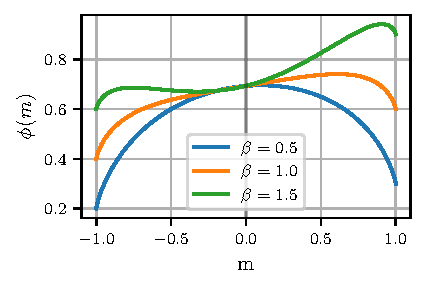
\includegraphics[width=0.49\textwidth]{curieweiss/m_phi_B01.pdf}
    \caption{The function $\phi(m)$ defined in Equation~\ref{eq:curie_weiss_phi} for $B=0$ (left) and $B=0.1$ (right).}
    \label{fig:curie_weiss_phi_B0}
\end{figure}

Using the laplace approximation, we see that the integral is dominated by the maximum of $\phi(m)$, which we will call $m_0$.

\begin{equation}
    \begin{gathered}
        \frac{d}{dm}\phi(m_0) =  0 \\
        \implies \beta J m_0 + \beta B + \frac{1}{2}\left(\log \frac{1-m}{1+m}\right) = 0\\
        \implies \arctanh(m_0) = \beta J m_0 + \beta B\\
    \end{gathered}
\end{equation}
Thus, we have found the mean-field equation for the Curie-Weiss model:
\begin{equation}
    \label{eq:curie_weiss_self_consistent}
    m = \tanh(\beta J m + \beta B)
\end{equation}
This equation is similar to the one we found for the Ising model in Equation~\ref{eq:ising}, however, this time we have a phase transition. In Figure~\ref{fig:curie_weiss_equation} we can see that, for different value of $\beta$, we can have one or three solutions to the equation. In the case of $B=0$, we can have one solution for $\beta < \beta_c$ and three solutions for $\beta > \beta_c$. The critical value of $\beta$ is given by:
\begin{equation}
    \beta_c = \frac{1}{J}
\end{equation}

\begin{figure}[h]
    \centering
    \begin{minipage}[t]{0.45\textwidth}
        \centering
        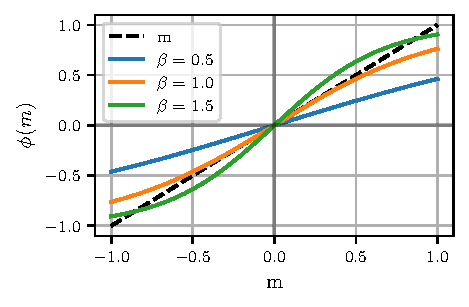
\includegraphics[width=\textwidth]{curieweiss/rhs_lhs.pdf}
        \caption{The left-hand side and right-hand side of Equation~\ref{eq:curie_weiss_self_consistent} for $B=0$ plotted for different values of $\beta$. Intersecting points correspond to solutions of the equation.}
        \label{fig:curie_weiss_equation}
    \end{minipage}
    \hfill
    \begin{minipage}[t]{0.45\textwidth}
        \centering
        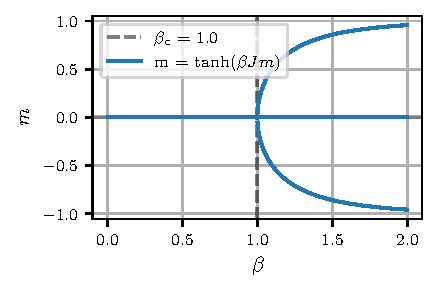
\includegraphics[width=\textwidth]{curieweiss/m_vs_beta.pdf}
        \caption{Solutions to Equation~\ref{eq:curie_weiss_self_consistent} with respect to the inverse temperature $\beta$ for $B=0$.}
        \label{fig:curie_weiss_solutions}
    \end{minipage}
\end{figure}
\chapter{The Bornholdt model}\label{ch:bornholdt_model}
In the spirit of finding a model for the price dynamics of risky assets, we now present the model proposed in \cite{bornholdt}. The idea is to formulate a model with maximum simplicity, which includes the possibility of strategic interaction between agents in the market.



\section{Introduction}
\subsection{Financial motivation}
In \cite{bornholdt}, a simple spin model, which we will refer to as the Bornholdt model, is proposed to model trading in financial markets. In the model, agents are seen as interacting spins, which have two possible actions: buy or sell an asset. The choice of each agent is influenced by two contrasting forces:
\begin{itemize}
    \item ``Do what your neighbors do'': this is the strategy that momentum traders follow. They try to follow the trend in the market, buying when the price is rising and selling when it is falling.
    \item ``Do what the minority does'': this is the strategy that mean-reversion traders follow. They try to buy when the price is falling and sell when it is rising, betting on a reversal of the trend.
\end{itemize}
We will see how these two strategies are implemented in the model.

\subsection{Model definition}
Consider a model with N spins with orientations $\sigma_i\in\{-1,+1\}$, representing the decision of agent $i$ to buy or sell a stock. We will consider updates following a heat-bath dynamics:
\begin{equation}
    \begin{aligned}
        \sigma_i(t+1) &= +1 \;\text{with }\; p = \frac{1}{1+e^{-2\beta h_i(t)}}\\
        \sigma_i(t+1) &= -1 \;\text{with }\; 1-p
    \end{aligned}
    \label{eq:heat_bath}
\end{equation}
Where $h_i(t)$ is the local field of agent $i$ at time $t$:
\begin{equation}
    h_i(t)=\sum_{j=1}^N J_{i j} \sigma_j-\alpha C_i(t) \frac{1}{N} \sum_{j=1}^N \sigma_j(t)
\end{equation}
Where $J_{i j}$ is the coupling between agents $i$ and $j$, $\sigma_j$ is the agent's action at $t$, $C_i(t)$ is the strategy of $i$ at time $t$, and $\alpha$ is a parameter. The first term in the local field pushes the agent to follow the trend of spins in their proximity (do what your neighbors do), while the second term pushes the agent to follow the minority (do what the minority does), assuming the strategy $C_i(t)$ is positive. 
If we consider the case in which $C_i(t) = 1\;\forall i, t$, we have that each trader follows both a momentum and a mean-reversion strategy simultaneously. This leads to near-vanishing magnetization even for temperatures below the critical temperature. 
We will focus on the more interesting and realistic case in which the strategies are updated at each time by each agent. Specifically, we will assume that a trader in the majority will try to switch to the minority strategy and thus adopt $C_i(t+1) = +1$, while a trader in the minority will try to switch to the majority strategy and thus adopt $C_i(t+1) = -1$. This is a reasonable assumption, as traders in the minority are likely to be more cautious and risk-averse, while traders in the majority are likely to be more aggressive and willing to take risks. This dynamics is the described by:
\begin{equation}
    C_i(t+1) = \begin{cases}
        +1 & \text{if} \quad \alpha\sigma_i(t) \sum_{j=1}^N \sigma_j(t)> 0\\
        -1 & \text{otherwise}
    \end{cases}
\end{equation}
Rearranging the equation, we can write:
\begin{equation}
    C_i(t+1) = \begin{cases}
        +C_i(t) & \text{if} \quad \alpha\sigma_i(t)C_i(t) \sum_{j=1}^N \sigma_j(t)> 0\\
        -C_i(t) & \text{otherwise}
    \end{cases}
\end{equation}
Now, we can take one extra step and assume that the strategy update is done instantaneously, so that we can write:
\begin{equation}
    C_i(t) = \begin{cases}
        +C_i(t) & \text{if} \quad \alpha\sigma_i(t)C_i(t) \sum_{j=1}^N \sigma_j(t)> 0\\
        -C_i(t) & \text{otherwise}
    \end{cases}
\end{equation}
Then, substituting this into the local field, we have a remarkably simple expression for the local field:
\begin{equation}
    h_i=\sum_{j=1}^N J_{i j} \sigma_j-\alpha \sigma_i \left | \frac{1}{N}\sum_{j=1}^N \sigma_j \right |
\end{equation}
Then, the hamiltonian of the model is:
\begin{equation}
    \begin{aligned}
        H(\underline{\sigma}) &= -\sum_{i=1}^N \sigma_i h_i\\
        &= -\sum_{i,j}J_{i,j}\sigma_i\sigma_j + \frac{\alpha}{N}\sum_{i=1}^N \sigma_i \left | \sum_{j=1}^N \sigma_j \right |
    \end{aligned}
\end{equation}
At this point, the magnetization \(M = \frac{1}{N}\sum_{j=1}^N \sigma_j\) can be interpreted as the price of the security that is being traded. We seek to study the dynamics of the model.

\subsection{Analysis of the model}
We will focus on the fully connected case in which \(J_{i,j}=\frac{J}{N} \; \forall i,j\). The hamiltonian of the model is then:
\begin{equation}
    H(\underline{\sigma}) = -\frac{J}{N}\sum_{i,j}\sigma_i\sigma_j + \frac{\alpha}{N}\sum_{i=1}^N \sigma_i \left | \sum_{j=1}^N \sigma_j \right |
\end{equation}

We will proceed in a similar way as in Section~\ref{sec:curie_weiss}, by introducing a combinatorial factor $\mathcal{N}(m)$ and taking the large $N$ limit.

The partition function of the model is given by:
\begin{equation}
    \begin{aligned}
        Z &= \sum_{\underline{\sigma}\in\mathcal{X}_N}e^{-\beta H(\underline{\sigma})}\\
        &= \sum_{\underline{\sigma}\in\mathcal{X}_N}e^{-\beta\frac{J}{N}\sum_{i,j}\sigma_i\sigma_j + \beta\frac{\alpha}{N}\sum_{i=1}^N \sigma_i \left | \sum_{j=1}^N \sigma_j \right |}\\
        &= \sum_{\underline{\sigma}\in\mathcal{X}_N}e^{-\beta\frac{J}{N}\left(\sum_{i}\sigma_i\right)^2 + \beta\frac{\alpha}{N}\sum_{i=1}^N \sigma_i \left | \sum_{j=1}^N \sigma_j \right |}\\
    \end{aligned}
\end{equation}
Now, we can introduce the notation:
\begin{equation}
m(\underline{\sigma}) = \frac{1}{N}\sum_{i}\sigma_i
\end{equation}
Then, we can rewrite the hamiltonian as:

\begin{equation}
    H(\underline{\sigma}) =  - J N m^2(\underline{\sigma}) + \alpha N m(\underline{\sigma}) \left| m(\underline{\sigma}) \right|
\end{equation}

And the partition function becomes:
\begin{equation}
    \begin{aligned}
        Z &= \sum_{\underline{\sigma}\in\mathcal{X}_N}e^{N\left(\beta J  m^2(\underline{\sigma})+\beta \alpha  m(\underline{\sigma}) \left| m(\underline{\sigma})\right|\right)}\\
        &= \sum_{m}e^{N\left(\beta J  m^2+\beta \alpha  m \left| m\right|\right)}\mathcal{N}(m)\\
        &= \sum_{m}e^{N\left(\beta J  m^2+\beta \alpha  m \left| m\right| + \frac{1}{N}\log \mathcal{N}(m)\right)}\\
    \end{aligned}
\end{equation}
Where $\mathcal{N}(m)$ is the number of configurations with magnetization $m$. In Section~\ref{sec:curie_weiss}, we have seen that $S(m) :=\lim_{N\rightarrow\infty}\frac{1}{N}\log \mathcal{N}(m)$ is the Shannon entropy of a bernoulli distribution with probability $p = \frac{1+m}{2}$ and $q = \frac{1-m}{2}$.

Then, in the large $N$ limit, we notice the following:
\begin{itemize}
    \item The increments of $m$ become infinitesimal, allowing us to treat the sum as an integral.
    \item We can subtitute $\frac{1}{N}\log\mathcal{N}(m)$ with $S(m)$.
\end{itemize}
Then, we can rewrite the partition function as:
\begin{equation}
    Z \approx \int_{-1}^{1} dm e^{N\phi(m)}, \quad \text{where }
    \phi(m) = \beta J m^2 + \alpha m |m| + S(m)
\end{equation}

We now aim to rewrite $\phi(m)$ in a more convenient form. First, we notice that:
\begin{equation}
    x|x| = x^2 (2\theta(x)-1)
\end{equation}
Where $\theta(x)$ is the Heaviside step function:
\begin{equation}
    \theta(x) = \begin{cases}
        0 & \text{if } x < 0\\
        1 & \text{if } x \geq 0
    \end{cases}
\end{equation}
Then, we can rewrite $\phi(m)$ as:
\begin{equation}
    \phi(m) = \beta J m^2 + \alpha m^2 (2\theta(m)-1) + S(m)
\end{equation}
\textcolor{red}{finish analysis of the model}

\section{Simulations of the Bornholdt model}
\textcolor{red}{fix plots}\\
We conducted an extensive numerical simulation of the Bornholdt model, employing a system consisting of 1024 spins arranged in a two-dimensional square lattice. The coupling constant was set to $J=1.0$, the external field parameter was $\alpha=4.0$, and the temperature of the system was defined as $T=1/\beta=1.5$. The simulation was carried out over a sufficiently large number of time steps to allow the results to be representative of the model's long-term dynamics.

\subsection{Only fundamental traders}
We start by analysing the case in which all agents are fundamental traders, meaning that they all follow the same strategy. In this case, we set $C_i(t) = 1$ for all agents and all times. The results of the simulation are shown in figure \ref{fig:fundamental_traders}. As expected, the system is stuck in a noisy state in which the magnetization fluctuates between low positive and negative values.

\begin{figure}[H]
    \centering
    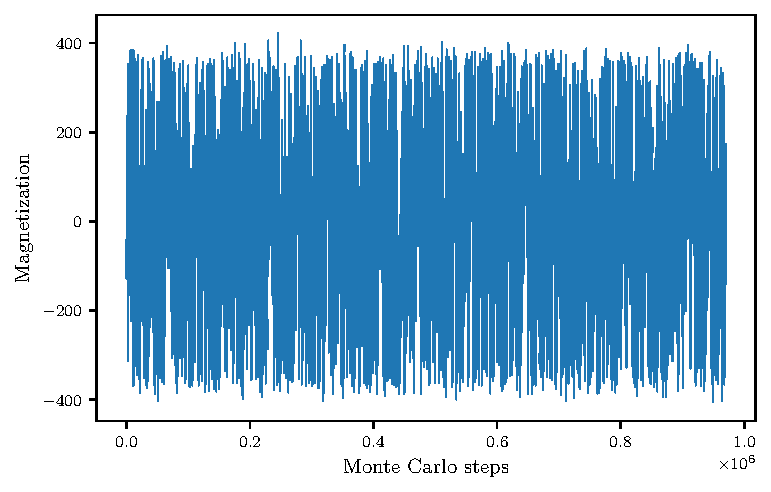
\includegraphics[width=0.9\textwidth]{constant_c_magnetization.pdf}
    \caption{Dynamics of the magnetization of the system with only fundamental traders.}
    \label{fig:fundamental_traders}
\end{figure}

\subsection{Dynamics of the strategies}
The simulations indicate that the initial distribution of agents' strategies has a negligible long-term impact on the system's behavior. Regardless of the starting configuration, the system quickly converges to a stable state where approximately 50\% to 70\% of agents adopt the strategy $C_i(t) = 1$. This convergence is evident from the dynamics shown in figure \ref{fig:strategies}. Consequently, for the purposes of simulating the model, it is not necessary to distinguish between different initial distributions of strategies, as the system's evolution is largely independent of these initial conditions.

\begin{figure}[H]
    \centering
    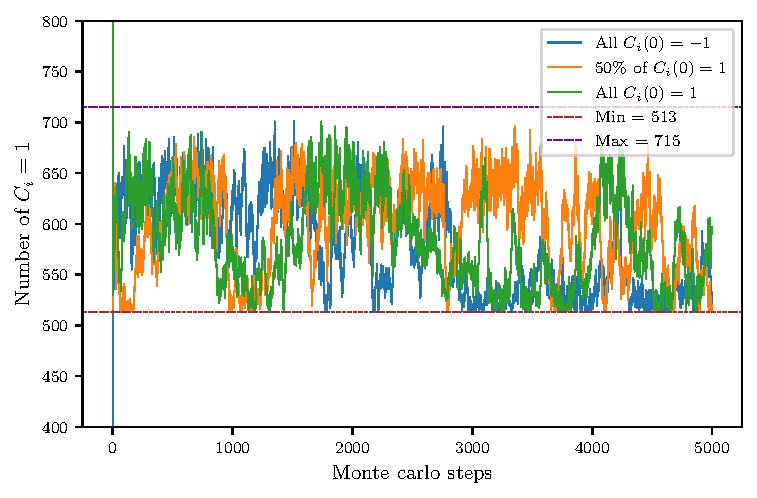
\includegraphics[width=0.9\textwidth]{c_values.pdf}
    \caption{Dynamics of agent's strategy based on different starting distributions.}
    \label{fig:strategies}
\end{figure}

\subsection{Dynamics of the price}
Following the interpretation proposed in \cite{bornholdt}, the magnetization of the system is treated as the price of a financial asset being traded by the agents. By plotting the magnetization as a function of time, we obtain a time-series that mimics the price dynamics of a financial asset. This is illustrated in figure \ref{fig:magnetization}, where the temporal evolution of the magnetization is shown.

In addition to examining the magnetization (i.e., the price), it is also insightful to analyze the underlying configuration of spins that produces this magnetization. The spin configuration provides a microscopic view of the system's state, which complements the macroscopic perspective offered by the magnetization. As shown in figure \ref{fig:lattices}, the system alternates between two distinct regimes: metastable states, where the spin configuration remains relatively stable over time, and turbulent states, characterized by rapid and chaotic changes in the spin configuration. These alternating regimes highlight the complex dynamics of the system and their influence on the observed price behavior.

\begin{figure}[H]
    \centering
    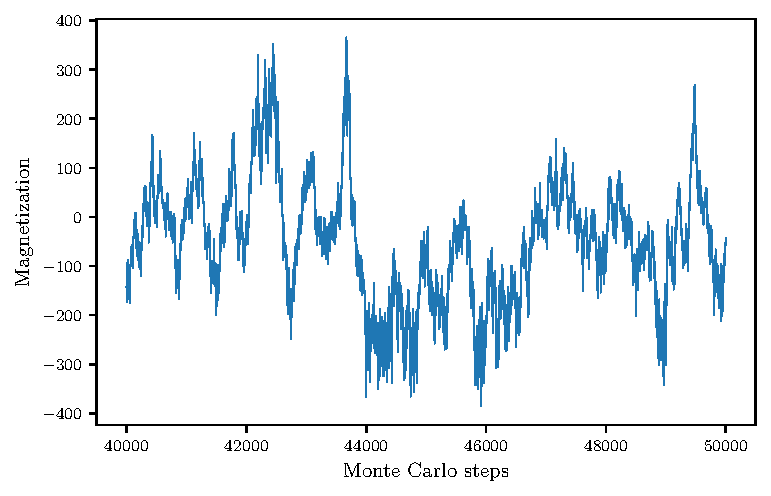
\includegraphics[width=0.9\textwidth]{magnetization.pdf}
    \caption{Dynamics of the magnetization of the system.}
    \label{fig:magnetization}
\end{figure}

\begin{figure}[H]
    \centering
    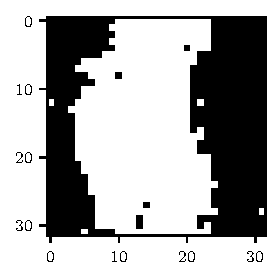
\includegraphics[width=0.3\textwidth]{lattices/metastable_turbulent/43400.pdf}
    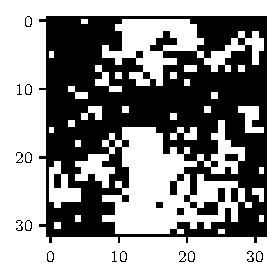
\includegraphics[width=0.3\textwidth]{lattices/metastable_turbulent/43700.pdf}
    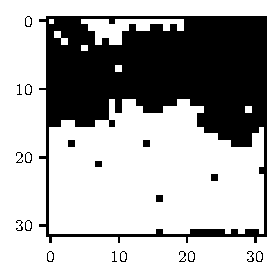
\includegraphics[width=0.3\textwidth]{lattices/metastable_turbulent/43850.pdf}
    \caption{Snapshots of the lattices at times $t=43400$, $t=43700$ and $t=43850$.}
    \label{fig:lattices}
\end{figure}

\subsection{Dynamics and statistical properties of the returns}
To analyze the dynamics of the returns of the asset, we define the log-returns as the logarithm of the ratio of the magnetization at consecutive time steps. Since the magnetization $M(t)$ can take on both positive and negative values, we use its absolute value to ensure that the log-returns are well-defined. Additionally, to avoid issues with division by zero or taking the logarithm of zero, we introduce a small positive constant $\epsilon$, where $\epsilon \ll 1$. The log-returns are then computed as:
\begin{equation}
    R(t) = \log\left(\frac{|M(t)| + \epsilon}{|M(t-1)| + \epsilon}\right)
\end{equation}
Here, $R(t)$ represents the return at time $t$, $M(t)$ is the magnetization at time $t$, and $\epsilon$ is a small constant added for numerical stability.

The resulting time-series of the returns is shown in figure \ref{fig:returns}.

\begin{figure}[H]
    \centering
    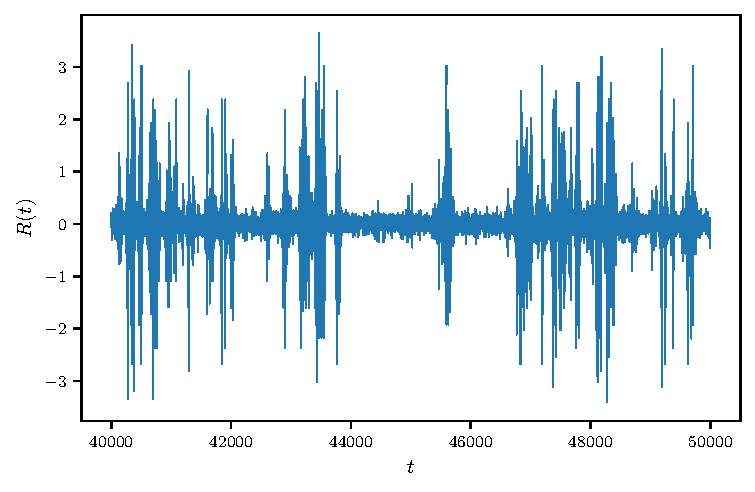
\includegraphics[width=0.9\textwidth]{returns.pdf}
    \caption{Time-series of the returns of the asset.}
    \label{fig:returns}
\end{figure}

From a financial perspective, we are interested in checking wether the returns exhibit the statistical properties of real financial data, namely fat tails and autocorrelation, as noted in \cite{bouchaud2000theory}.

\subsubsection{Fat tails}
The analysis of the distribution of the returns, as illustrated in figures \ref{fig:returns_distribution} and \ref{fig:cumulative_returns_distribution}, provides strong evidence that the returns exhibit fat tails. This characteristic is a hallmark of financial time-series and indicates that extreme events (large positive or negative returns) occur more frequently than would be expected under a normal distribution.

To further investigate this property, we compare the returns to a normal distribution using a QQ-plot, shown in figure \ref{fig:qqplot}. The QQ-plot clearly demonstrates significant deviations from the straight line that would be expected if the returns were normally distributed. These deviations, particularly in the tails, confirm the presence of fat tails in the distribution.

Additionally, we perform a statistical test to formally assess whether the returns follow a normal distribution. Specifically, we use the Shapiro-Wilk test, which tests the null hypothesis that the data is drawn from a normal distribution. The results of the test yield a p-value on the order of $10^{-192}$. Such an extremely small p-value indicates that we can reject the null hypothesis with extremely high confidence, confirming that the returns are not normally distributed. Additionally, we compute the kurtosis of the returns, which is approximately 24.2. This value indicates an extremely leptokurtic distribution, suggesting a very high likelihood of outliers.
\begin{figure}[H]
    \centering
    \begin{minipage}[T]{0.45\textwidth}
        \centering
        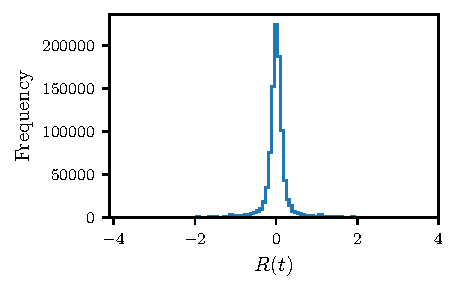
\includegraphics[width=\textwidth]{distribution_returns.pdf}
        \caption{Distribution of the returns of the asset.}
        \label{fig:returns_distribution}
    \end{minipage}
    \hfill
    \begin{minipage}[T]{0.45\textwidth}
        \centering
        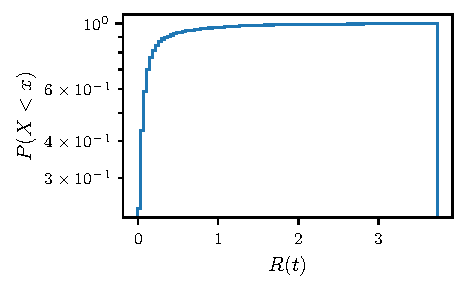
\includegraphics[width=\textwidth]{cumulative_distribution.pdf}
        \caption{Cumulative distribution of the returns of the asset.}
        \label{fig:cumulative_returns_distribution}
    \end{minipage}
\end{figure}


\subsubsection{Autocorrelation}
From figure \ref{fig:returns}, we can already seen that the periods of high volatility (i.e. large positive or negative returns) tend to be clustered together. This is a sign of autocorrelation in the returns. To quantify this, we can compute the autocorrelation function of the returns, defined as
\begin{equation}
    \rho(k) = \frac{\sum_{t=1}^{N-k} (R(t) - \bar{R})(R(t+k) - \bar{R})}{\sum_{t=1}^{N} (R(t) - \bar{R})^2}
\end{equation}
where $N$ is the number of returns, $R(t)$ is the return at time $t$, and $\bar{R}$ is the mean of the returns. The autocorrelation function measures the correlation between the returns at time $t$ and time $t+k$. A positive value of $\rho(k)$ indicates that the returns at time $t$ and time $t+k$ are positively correlated, while a negative value indicates that they are negatively correlated. A value close to zero indicates that there is no correlation between the returns at time $t$ and time $t+k$.
The autocorrelation function is computed for lags $k=1,2,\ldots,100$ and is shown in figure \ref{fig:autocorrelation}. The results show that the autocorrelation is significant for a large number of lags, which is consistent with the empirical observation that financial returns are autocorrelated.

\begin{figure}[H]
    \centering
    \begin{minipage}[T]{0.45\textwidth}
        \centering
        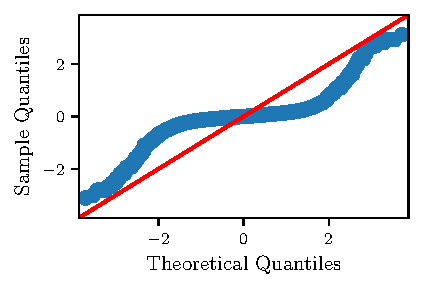
\includegraphics[width=\textwidth]{qqplot-returns.pdf}
        \caption{QQ-plot of the returns against a normal distribution.}
        \label{fig:qqplot}
    \end{minipage}
    \hfill
    \begin{minipage}[T]{0.45\textwidth}
        \centering
        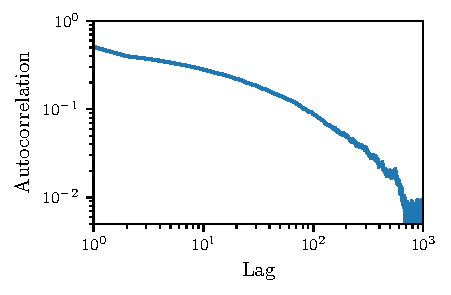
\includegraphics[width=\textwidth]{autocorrelation.pdf}
        \caption{Autocorrelation function of the returns.}
        \label{fig:autocorrelation}
    \end{minipage}
\end{figure}


\section{Discussion}
The results of the simulation suggest that the Bornholdt model is able to reproduce some of the statistical properties of real financial data, such as fat tails and autocorrelation of returns. This is interesting because the model is based on a simple spin model, and does not rely on any assumptions about the rationality of agents or the efficiency of markets.

As seen in \ref{sec:financial_background}, one of the main assumptions of the model introduced in \cite{black_scholes} is that the price of the underlying asset follows a geometric Brownian motion. The Bornholdt model, however, results in price dynamics which exhibit fat tails, and do not have independent increments, as shown by the autocorrelation of the returns, which is the case also in real financial data.

The key observation here is that, unlike in a geometric Brownian motion, the price (i.e. magnetization) at time $t$ is not enough to describe the distribution of prices at times $t+s, \; s\geq 0$. This might be counterintuitive, as by equation \ref{eq:heat_bath}, the future configuration of spins is determined by the current configuration of spins. However, it is important to note that the current magnetization is not enough to determine the current configuration of spins. In fact, the magnetization is a global property of the system, while the configuration can vary locally. In figures \ref{fig:lattices_m100} and \ref{fig:magnetization_m100}, we can see that the magnetization is the same at times $t=129722$ and $t=130293$, but the configuration of spins is completely different.

\begin{figure}[H]
    \centering
    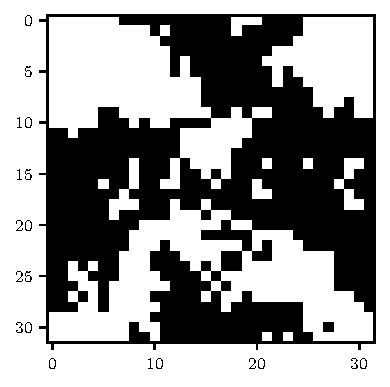
\includegraphics[width=0.4\textwidth]{lattices/same_magnetization/129722.pdf}
    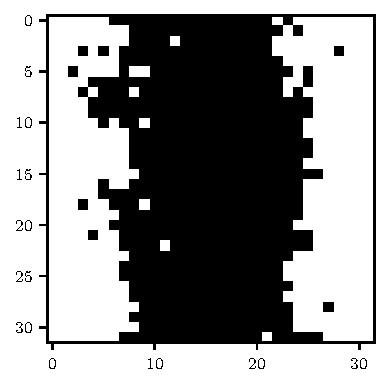
\includegraphics[width=0.4\textwidth]{lattices/same_magnetization/130293.pdf}
    \caption{Snapshots of the lattices at times $t=129722$, and $t=130293$.}
    \label{fig:lattices_m100}
\end{figure}

\begin{figure}[H]
    \centering
    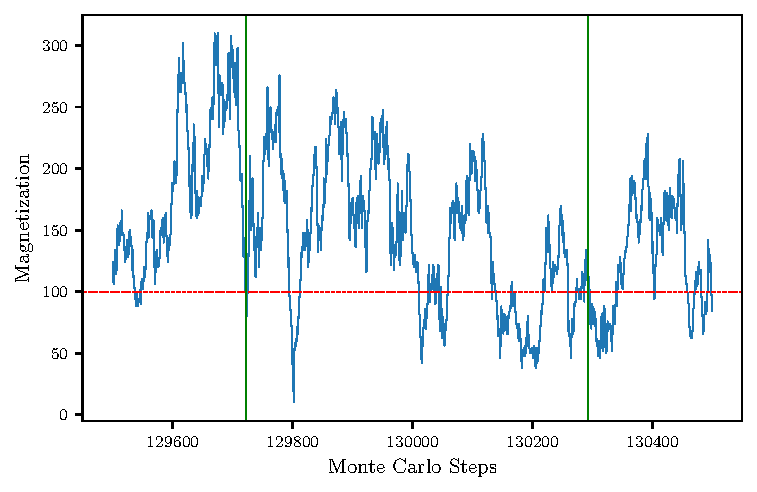
\includegraphics[width=0.9\textwidth]{lattices/same_magnetization/magnetization.pdf}
    \caption{Dynamics of the magnetization of the system. The green lines represent the times at which the snapshots in figure \ref{fig:lattices_m100} were taken.} \textcolor{red}{fix plot}
    \label{fig:magnetization_m100}
\end{figure}
\chapter{Conclusion}\label{ch:conclusion}
In this thesis, we have explored [briefly summarize the main topics or findings]. The results indicate that [summarize key findings]. 

The contributions of this work include [list contributions]. Future work could focus on [suggest future research directions].


\bibliographystyle{apalike}
\bibliography{bibliography.bib}

Unless otherwise stated, all figures are created by the author. Figure \ref{fig:ising_model} is adapted from the original by Ta2o, CC BY 4.0, via Wikimedia Commons \url{https://upload.wikimedia.org/wikipedia/commons/f/fe/2D_ising_model_on_lattice.svg}


\end{document}